\documentclass{book}
\usepackage[a4paper,top=2.5cm,bottom=2.5cm,left=2.5cm,right=2.5cm]{geometry}
\usepackage{makeidx}
\usepackage{natbib}
\usepackage{graphicx}
\usepackage{multicol}
\usepackage{float}
\usepackage{listings}
\usepackage{color}
\usepackage{ifthen}
\usepackage[table]{xcolor}
\usepackage{textcomp}
\usepackage{alltt}
\usepackage{ifpdf}
\ifpdf
\usepackage[pdftex,
            pagebackref=true,
            colorlinks=true,
            linkcolor=blue,
            unicode
           ]{hyperref}
\else
\usepackage[ps2pdf,
            pagebackref=true,
            colorlinks=true,
            linkcolor=blue,
            unicode
           ]{hyperref}
\usepackage{pspicture}
\fi
\usepackage[utf8]{inputenc}
\usepackage{mathptmx}
\usepackage[scaled=.90]{helvet}
\usepackage{courier}
\usepackage{sectsty}
\usepackage{amssymb}
\usepackage[titles]{tocloft}
\usepackage{doxygen}
\lstset{language=C++,inputencoding=utf8,basicstyle=\footnotesize,breaklines=true,breakatwhitespace=true,tabsize=4,numbers=left }
\makeindex
\setcounter{tocdepth}{3}
\renewcommand{\footrulewidth}{0.4pt}
\renewcommand{\familydefault}{\sfdefault}
\hfuzz=15pt
\setlength{\emergencystretch}{15pt}
\hbadness=750
\tolerance=750
\begin{document}
\hypersetup{pageanchor=false,citecolor=blue}
\begin{titlepage}
\vspace*{7cm}
\begin{center}
{\Large Draw it! }\\
\vspace*{1cm}
{\large Generated by Doxygen 1.8.2}\\
\vspace*{0.5cm}
{\small Mon Sep 2 2013 20:54:50}\\
\end{center}
\end{titlepage}
\clearemptydoublepage
\pagenumbering{roman}
\tableofcontents
\clearemptydoublepage
\pagenumbering{arabic}
\hypersetup{pageanchor=true,citecolor=blue}
\chapter{draw-\/it}
\label{md_README}
\hypertarget{md_README}{}
This program is going to be able to recognize drawn Jump'n'Run levels on photos with Open\-C\-V and convert them so that a simple Jump'n'Run game programmed in S\-F\-M\-L will be able to use it.

\section*{How to build }

This program is currently developed with the I\-D\-E Q\-T-\/\-Creator and qmake, which uses a .pro file for build configuration. If you want to build the program with another I\-D\-E or maybe command line, the following is required\-:
\begin{DoxyItemize}
\item The Open\-C\-V library and header files (I am using version 2.\-4.\-6)
\item The S\-F\-M\-L library and header files (I am using version 2.\-1)
\item A c++11 compatible c++ compiler (I am using the g++ which is part of the gcc) I havent't build the program without Qt-\/\-Creator yet, so I can't give you any further information.
\end{DoxyItemize}

\section*{Building the Documentation }

If you want to create the documentation yourself, which is included in the source code, you need the tool 'doxygen' (\href{http://www.stack.nl/~dimitri/doxygen/}{\tt http\-://www.\-stack.\-nl/$\sim$dimitri/doxygen/}). A config file is alreay included in the repo. Just run doxygen like 'doxygen config' and there is a documentation in html and latex created. 
\chapter{Hierarchical Index}
\section{Class Hierarchy}
This inheritance list is sorted roughly, but not completely, alphabetically\-:\begin{DoxyCompactList}
\item Drawable\begin{DoxyCompactList}
\item \contentsline{section}{tile\-Map}{\pageref{classtileMap}}{}
\end{DoxyCompactList}
\item \contentsline{section}{Entities}{\pageref{classEntities}}{}
\begin{DoxyCompactList}
\item \contentsline{section}{Player}{\pageref{classPlayer}}{}
\end{DoxyCompactList}
\item \contentsline{section}{Game}{\pageref{classGame}}{}
\item \contentsline{section}{Line\-Finder}{\pageref{classLineFinder}}{}
\item \contentsline{section}{Play}{\pageref{classPlay}}{}
\item Q\-Main\-Window\begin{DoxyCompactList}
\item \contentsline{section}{Main\-Window}{\pageref{classMainWindow}}{}
\end{DoxyCompactList}
\item Q\-Widget\begin{DoxyCompactList}
\item \contentsline{section}{Q\-S\-F\-M\-L\-Canvas}{\pageref{classQSFMLCanvas}}{}
\begin{DoxyCompactList}
\item \contentsline{section}{my\-Canvas}{\pageref{classmyCanvas}}{}
\end{DoxyCompactList}
\end{DoxyCompactList}
\item Render\-Window\begin{DoxyCompactList}
\item \contentsline{section}{Q\-S\-F\-M\-L\-Canvas}{\pageref{classQSFMLCanvas}}{}
\end{DoxyCompactList}
\item Transformable\begin{DoxyCompactList}
\item \contentsline{section}{tile\-Map}{\pageref{classtileMap}}{}
\end{DoxyCompactList}
\end{DoxyCompactList}

\chapter{Class Index}
\section{Class List}
Here are the classes, structs, unions and interfaces with brief descriptions\-:\begin{DoxyCompactList}
\item\contentsline{section}{\hyperlink{classEntities}{Entities} \\*The entities class }{\pageref{classEntities}}{}
\item\contentsline{section}{\hyperlink{classGame}{Game} }{\pageref{classGame}}{}
\item\contentsline{section}{\hyperlink{classLineFinder}{Line\-Finder} }{\pageref{classLineFinder}}{}
\item\contentsline{section}{\hyperlink{classMainWindow}{Main\-Window} }{\pageref{classMainWindow}}{}
\item\contentsline{section}{\hyperlink{classmyCanvas}{my\-Canvas} }{\pageref{classmyCanvas}}{}
\item\contentsline{section}{\hyperlink{classPlay}{Play} \\*The \hyperlink{classPlay}{Play} class }{\pageref{classPlay}}{}
\item\contentsline{section}{\hyperlink{classPlayer}{Player} }{\pageref{classPlayer}}{}
\item\contentsline{section}{\hyperlink{classQSFMLCanvas}{Q\-S\-F\-M\-L\-Canvas} }{\pageref{classQSFMLCanvas}}{}
\item\contentsline{section}{\hyperlink{classtileMap}{tile\-Map} \\*The \hyperlink{classtileMap}{tile\-Map} class }{\pageref{classtileMap}}{}
\end{DoxyCompactList}

\chapter{File Index}
\section{File List}
Here is a list of all files with brief descriptions\-:\begin{DoxyCompactList}
\item\contentsline{section}{\hyperlink{entities_8cpp}{entities.\-cpp} }{\pageref{entities_8cpp}}{}
\item\contentsline{section}{\hyperlink{entities_8hpp}{entities.\-hpp} }{\pageref{entities_8hpp}}{}
\item\contentsline{section}{\hyperlink{errcodes_8h}{errcodes.\-h} }{\pageref{errcodes_8h}}{}
\item\contentsline{section}{\hyperlink{game_8cpp}{game.\-cpp} }{\pageref{game_8cpp}}{}
\item\contentsline{section}{\hyperlink{game_8hpp}{game.\-hpp} }{\pageref{game_8hpp}}{}
\item\contentsline{section}{\hyperlink{linefinder_8cpp}{linefinder.\-cpp} }{\pageref{linefinder_8cpp}}{}
\item\contentsline{section}{\hyperlink{linefinder_8hpp}{linefinder.\-hpp} }{\pageref{linefinder_8hpp}}{}
\item\contentsline{section}{\hyperlink{main_8cpp}{main.\-cpp} }{\pageref{main_8cpp}}{}
\item\contentsline{section}{\hyperlink{play_8cpp}{play.\-cpp} }{\pageref{play_8cpp}}{}
\item\contentsline{section}{\hyperlink{play_8hpp}{play.\-hpp} }{\pageref{play_8hpp}}{}
\end{DoxyCompactList}

\chapter{Class Documentation}
\hypertarget{classEntities}{\section{Entities Class Reference}
\label{classEntities}\index{Entities@{Entities}}
}


The entities class.  




{\ttfamily \#include $<$entities.\-hpp$>$}

Inheritance diagram for Entities\-:\begin{figure}[H]
\begin{center}
\leavevmode
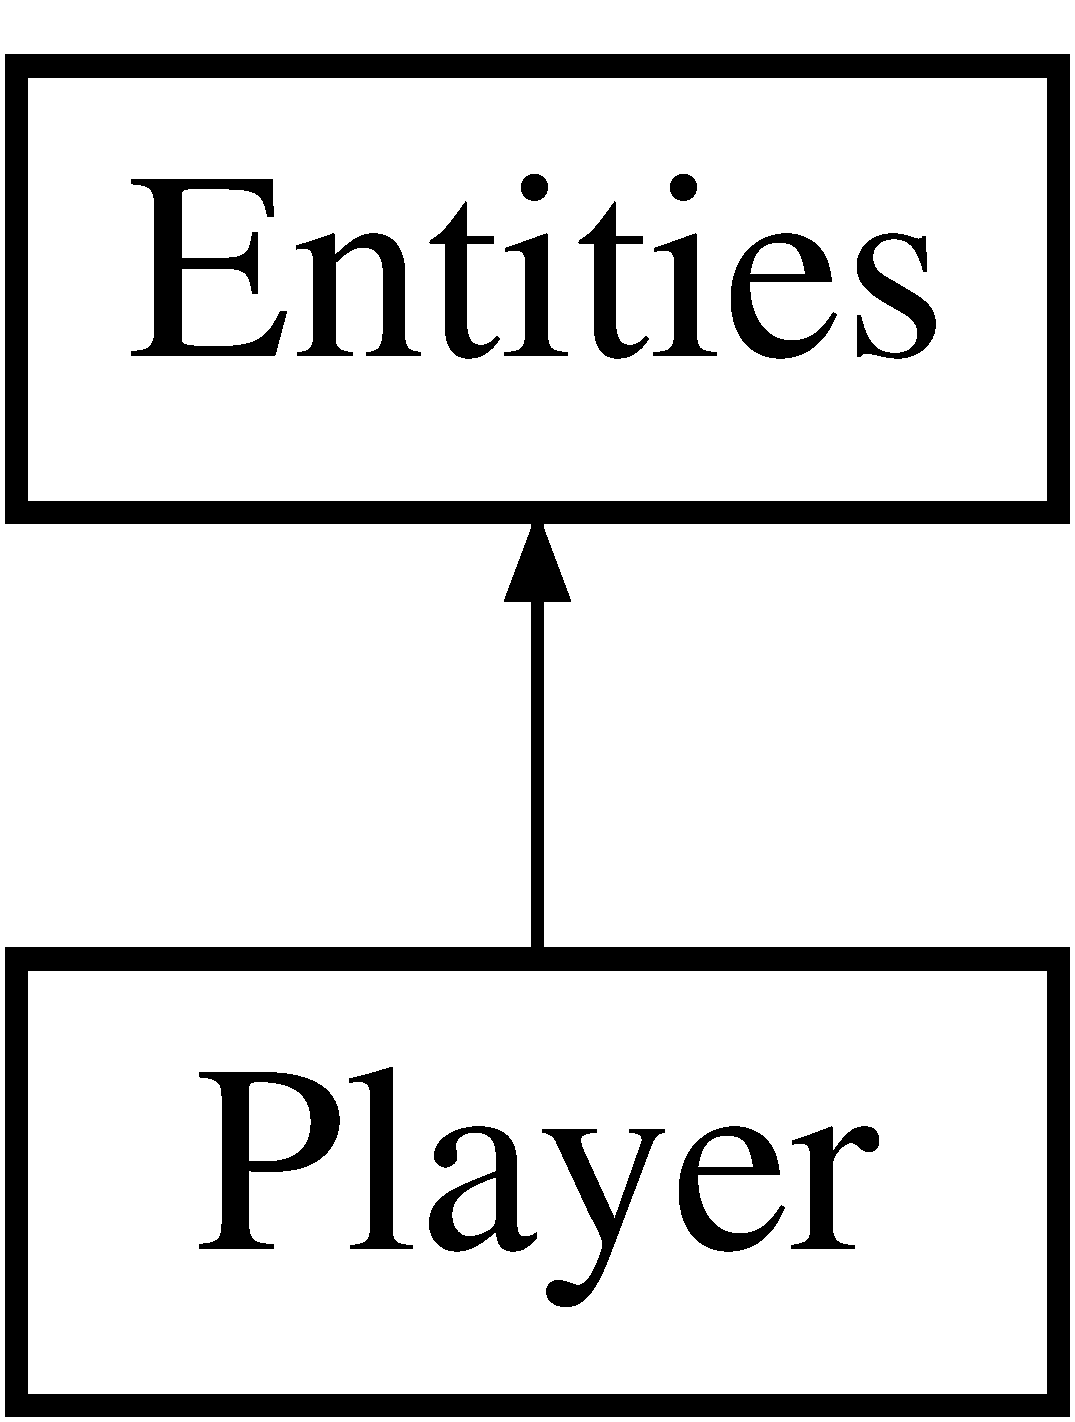
\includegraphics[height=2.000000cm]{classEntities}
\end{center}
\end{figure}
\subsection*{Public Member Functions}
\begin{DoxyCompactItemize}
\item 
\hyperlink{classEntities_a0632e3790f40fec4e831800d48ff491b}{Entities} ()
\item 
\hyperlink{classEntities_af131357f6b31e9e9bec551a5afa57dbd}{Entities} (sf\-::\-Vector2f pos)
\item 
\hyperlink{classEntities_a2b523e8705f7a102b466efad8d3162ba}{Entities} (float px, float py)
\item 
virtual \hyperlink{classEntities_ab0c6d116edff7d71de53252e99288825}{$\sim$\-Entities} ()
\item 
virtual void \hyperlink{classEntities_a10bf20192cbd1316f6b743aa2f4344ec}{set\-Position} (sf\-::\-Vector2f pos)
\item 
virtual void \hyperlink{classEntities_a86f93c9f2b2ece831234f274554de431}{set\-Position} (float px, float py)
\item 
virtual sf\-::\-Vector2f \hyperlink{classEntities_a7cf4315e835d2a68b91151f32fddeff7}{get\-Position} () const 
\item 
virtual void \hyperlink{classEntities_a2629ebdd7a4538f9686e812c58c21b41}{move} (sf\-::\-Vector2f movement)
\end{DoxyCompactItemize}


\subsection{Detailed Description}
The entities class. 

This is a base class for different entities appearing in the game. It only specifies common attributes. 

\subsection{Constructor \& Destructor Documentation}
\hypertarget{classEntities_a0632e3790f40fec4e831800d48ff491b}{\index{Entities@{Entities}!Entities@{Entities}}
\index{Entities@{Entities}!Entities@{Entities}}
\subsubsection[{Entities}]{\setlength{\rightskip}{0pt plus 5cm}Entities\-::\-Entities (
\begin{DoxyParamCaption}
{}
\end{DoxyParamCaption}
)}}\label{classEntities_a0632e3790f40fec4e831800d48ff491b}
\hypertarget{classEntities_af131357f6b31e9e9bec551a5afa57dbd}{\index{Entities@{Entities}!Entities@{Entities}}
\index{Entities@{Entities}!Entities@{Entities}}
\subsubsection[{Entities}]{\setlength{\rightskip}{0pt plus 5cm}Entities\-::\-Entities (
\begin{DoxyParamCaption}
\item[{sf\-::\-Vector2f}]{pos}
\end{DoxyParamCaption}
)}}\label{classEntities_af131357f6b31e9e9bec551a5afa57dbd}
\hypertarget{classEntities_a2b523e8705f7a102b466efad8d3162ba}{\index{Entities@{Entities}!Entities@{Entities}}
\index{Entities@{Entities}!Entities@{Entities}}
\subsubsection[{Entities}]{\setlength{\rightskip}{0pt plus 5cm}Entities\-::\-Entities (
\begin{DoxyParamCaption}
\item[{float}]{px, }
\item[{float}]{py}
\end{DoxyParamCaption}
)}}\label{classEntities_a2b523e8705f7a102b466efad8d3162ba}
\hypertarget{classEntities_ab0c6d116edff7d71de53252e99288825}{\index{Entities@{Entities}!$\sim$\-Entities@{$\sim$\-Entities}}
\index{$\sim$\-Entities@{$\sim$\-Entities}!Entities@{Entities}}
\subsubsection[{$\sim$\-Entities}]{\setlength{\rightskip}{0pt plus 5cm}Entities\-::$\sim$\-Entities (
\begin{DoxyParamCaption}
{}
\end{DoxyParamCaption}
)\hspace{0.3cm}{\ttfamily [virtual]}}}\label{classEntities_ab0c6d116edff7d71de53252e99288825}


\subsection{Member Function Documentation}
\hypertarget{classEntities_a7cf4315e835d2a68b91151f32fddeff7}{\index{Entities@{Entities}!get\-Position@{get\-Position}}
\index{get\-Position@{get\-Position}!Entities@{Entities}}
\subsubsection[{get\-Position}]{\setlength{\rightskip}{0pt plus 5cm}sf\-::\-Vector2f Entities\-::get\-Position (
\begin{DoxyParamCaption}
{}
\end{DoxyParamCaption}
) const\hspace{0.3cm}{\ttfamily [virtual]}}}\label{classEntities_a7cf4315e835d2a68b91151f32fddeff7}
\hypertarget{classEntities_a2629ebdd7a4538f9686e812c58c21b41}{\index{Entities@{Entities}!move@{move}}
\index{move@{move}!Entities@{Entities}}
\subsubsection[{move}]{\setlength{\rightskip}{0pt plus 5cm}void Entities\-::move (
\begin{DoxyParamCaption}
\item[{sf\-::\-Vector2f}]{movement}
\end{DoxyParamCaption}
)\hspace{0.3cm}{\ttfamily [virtual]}}}\label{classEntities_a2629ebdd7a4538f9686e812c58c21b41}
\hypertarget{classEntities_a10bf20192cbd1316f6b743aa2f4344ec}{\index{Entities@{Entities}!set\-Position@{set\-Position}}
\index{set\-Position@{set\-Position}!Entities@{Entities}}
\subsubsection[{set\-Position}]{\setlength{\rightskip}{0pt plus 5cm}void Entities\-::set\-Position (
\begin{DoxyParamCaption}
\item[{sf\-::\-Vector2f}]{pos}
\end{DoxyParamCaption}
)\hspace{0.3cm}{\ttfamily [virtual]}}}\label{classEntities_a10bf20192cbd1316f6b743aa2f4344ec}
\hypertarget{classEntities_a86f93c9f2b2ece831234f274554de431}{\index{Entities@{Entities}!set\-Position@{set\-Position}}
\index{set\-Position@{set\-Position}!Entities@{Entities}}
\subsubsection[{set\-Position}]{\setlength{\rightskip}{0pt plus 5cm}void Entities\-::set\-Position (
\begin{DoxyParamCaption}
\item[{float}]{px, }
\item[{float}]{py}
\end{DoxyParamCaption}
)\hspace{0.3cm}{\ttfamily [virtual]}}}\label{classEntities_a86f93c9f2b2ece831234f274554de431}


The documentation for this class was generated from the following files\-:\begin{DoxyCompactItemize}
\item 
\hyperlink{entities_8hpp}{entities.\-hpp}\item 
\hyperlink{entities_8cpp}{entities.\-cpp}\end{DoxyCompactItemize}

\hypertarget{classGame}{\section{Game Class Reference}
\label{classGame}\index{Game@{Game}}
}


{\ttfamily \#include $<$game.\-hpp$>$}

\subsection*{Public Member Functions}
\begin{DoxyCompactItemize}
\item 
\hyperlink{classGame_ad59df6562a58a614fda24622d3715b65}{Game} ()
\item 
int \hyperlink{classGame_a99fb161fbbe87d25a8b73265a0611e58}{run} ()
\begin{DoxyCompactList}\small\item\em In this function the game action happens. \end{DoxyCompactList}\end{DoxyCompactItemize}


\subsection{Constructor \& Destructor Documentation}
\hypertarget{classGame_ad59df6562a58a614fda24622d3715b65}{\index{Game@{Game}!Game@{Game}}
\index{Game@{Game}!Game@{Game}}
\subsubsection[{Game}]{\setlength{\rightskip}{0pt plus 5cm}Game\-::\-Game (
\begin{DoxyParamCaption}
{}
\end{DoxyParamCaption}
)}}\label{classGame_ad59df6562a58a614fda24622d3715b65}


\subsection{Member Function Documentation}
\hypertarget{classGame_a99fb161fbbe87d25a8b73265a0611e58}{\index{Game@{Game}!run@{run}}
\index{run@{run}!Game@{Game}}
\subsubsection[{run}]{\setlength{\rightskip}{0pt plus 5cm}int Game\-::run (
\begin{DoxyParamCaption}
{}
\end{DoxyParamCaption}
)}}\label{classGame_a99fb161fbbe87d25a8b73265a0611e58}


In this function the game action happens. 

\begin{DoxyReturn}{Returns}
Error/\-Success code. 
\end{DoxyReturn}


The documentation for this class was generated from the following files\-:\begin{DoxyCompactItemize}
\item 
\hyperlink{game_8hpp}{game.\-hpp}\item 
\hyperlink{game_8cpp}{game.\-cpp}\end{DoxyCompactItemize}

\hypertarget{classLineFinder}{\section{Line\-Finder Class Reference}
\label{classLineFinder}\index{Line\-Finder@{Line\-Finder}}
}


{\ttfamily \#include $<$linefinder.\-hpp$>$}

\subsection*{Public Member Functions}
\begin{DoxyCompactItemize}
\item 
\hyperlink{classLineFinder_ac9a83317df7ff3d74a9add150962e849}{Line\-Finder} ()
\item 
void \hyperlink{classLineFinder_a4ffb60e7c12143a6824b884239243da9}{set\-Acc\-Resolution} (double d\-Rho, double d\-Theta)
\item 
void \hyperlink{classLineFinder_af76de2e78cc28b37fd15652e2967e56b}{set\-Min\-Vote} (int minv)
\item 
void \hyperlink{classLineFinder_a7655dc9adfaca75ed92c585d226a60df}{set\-Line\-Length\-And\-Gap} (double length, double gap)
\item 
cv\-::\-Mat \& \hyperlink{classLineFinder_abd5e230f01feaecbc0f138ee3da504bf}{get\-Image} ()
\item 
std\-::vector$<$ cv\-::\-Vec4i $>$ \hyperlink{classLineFinder_a2769bdd5845ce23539d6abce15aa0814}{get\-Lines} ()
\begin{DoxyCompactList}\small\item\em Access the detected lines. \end{DoxyCompactList}\item 
int \hyperlink{classLineFinder_a238c97d0b07eae22b1dcce4201309771}{set\-Image} (std\-::string file\-Path)
\item 
int \hyperlink{classLineFinder_a798b342c3ac2cc0f20145b16761ff701}{set\-Image} (cv\-::\-Mat image)
\item 
std\-::vector$<$ cv\-::\-Vec4i $>$ \hyperlink{classLineFinder_a7f516bf30904fa0037d19ab1d6306c15}{find\-Lines} ()
\item 
void \hyperlink{classLineFinder_a538e8d3ab154e53bdbe379f55c322530}{draw\-Detected\-Lines} (cv\-::\-Scalar color=cv\-::\-Scalar(255, 255, 255))
\item 
std\-::vector$<$ cv\-::\-Vec4i $>$ \hyperlink{classLineFinder_a4fe5f72054ba400611549ea25c25904e}{refine\-Detected\-Lines} (float min\-Difference=0.\-05f)
\item 
void \hyperlink{classLineFinder_ac075a64fd7e52769fae9b78c337e00e1}{create\-Skeleton} (int threshold=127)
\begin{DoxyCompactList}\small\item\em Creates a refined image by removing outer pixels of the structures in the image. \end{DoxyCompactList}\item 
std\-::vector$<$ std\-::vector$<$ int $>$ $>$ \hyperlink{classLineFinder_a16d011cf00154adb96a37a75773017dc}{save\-To\-Vec} ()
\begin{DoxyCompactList}\small\item\em Stores the image in a format S\-F\-M\-L can read for further processing. \end{DoxyCompactList}\item 
void \hyperlink{classLineFinder_af42fca457731b5911f4b9787f5ad0b15}{draw\-Line\-Points} ()
\begin{DoxyCompactList}\small\item\em Draws the beginning and the ending of a detected line on the original image. For debugging purposes. \end{DoxyCompactList}\end{DoxyCompactItemize}


\subsection{Constructor \& Destructor Documentation}
\hypertarget{classLineFinder_ac9a83317df7ff3d74a9add150962e849}{\index{Line\-Finder@{Line\-Finder}!Line\-Finder@{Line\-Finder}}
\index{Line\-Finder@{Line\-Finder}!LineFinder@{Line\-Finder}}
\subsubsection[{Line\-Finder}]{\setlength{\rightskip}{0pt plus 5cm}Line\-Finder\-::\-Line\-Finder (
\begin{DoxyParamCaption}
{}
\end{DoxyParamCaption}
)}}\label{classLineFinder_ac9a83317df7ff3d74a9add150962e849}


\subsection{Member Function Documentation}
\hypertarget{classLineFinder_ac075a64fd7e52769fae9b78c337e00e1}{\index{Line\-Finder@{Line\-Finder}!create\-Skeleton@{create\-Skeleton}}
\index{create\-Skeleton@{create\-Skeleton}!LineFinder@{Line\-Finder}}
\subsubsection[{create\-Skeleton}]{\setlength{\rightskip}{0pt plus 5cm}void Line\-Finder\-::create\-Skeleton (
\begin{DoxyParamCaption}
\item[{int}]{threshold = {\ttfamily 127}}
\end{DoxyParamCaption}
)}}\label{classLineFinder_ac075a64fd7e52769fae9b78c337e00e1}


Creates a refined image by removing outer pixels of the structures in the image. 

\begin{DoxyAuthor}{Author}
zemann
\end{DoxyAuthor}
The function makes sure that the image is grayscale, then applies a inverted threshold on it to obtain a binary image. In a loop, which ends when all pixels of the image are zero, the image is opened to remove unneccessary pixels, then this opened image is subtracted from the original image, which is in return copied to skeleton. At last, the image is eroded. This then is the starting image for the next iteration. The skeleton is returned. The function is based on this blog entry\-: \href{http://felix.abecassis.me/2011/09/opencv-morphological-skeleton}{\tt http\-://felix.\-abecassis.\-me/2011/09/opencv-\/morphological-\/skeleton}


\begin{DoxyParams}{Parameters}
{\em threshold\mbox{[}in\mbox{]},\-:} & optional parameter for specifing the threshold limit. The mode is always T\-H\-R\-E\-S\-H\-\_\-\-B\-I\-N\-A\-R\-Y.\\
\hline
\end{DoxyParams}
\begin{DoxyReturn}{Returns}
The created skeleton image. 
\end{DoxyReturn}
\hypertarget{classLineFinder_a538e8d3ab154e53bdbe379f55c322530}{\index{Line\-Finder@{Line\-Finder}!draw\-Detected\-Lines@{draw\-Detected\-Lines}}
\index{draw\-Detected\-Lines@{draw\-Detected\-Lines}!LineFinder@{Line\-Finder}}
\subsubsection[{draw\-Detected\-Lines}]{\setlength{\rightskip}{0pt plus 5cm}void Line\-Finder\-::draw\-Detected\-Lines (
\begin{DoxyParamCaption}
\item[{cv\-::\-Scalar}]{color = {\ttfamily cv\-:\-:Scalar(255,~255,~255)}}
\end{DoxyParamCaption}
)}}\label{classLineFinder_a538e8d3ab154e53bdbe379f55c322530}
\hypertarget{classLineFinder_af42fca457731b5911f4b9787f5ad0b15}{\index{Line\-Finder@{Line\-Finder}!draw\-Line\-Points@{draw\-Line\-Points}}
\index{draw\-Line\-Points@{draw\-Line\-Points}!LineFinder@{Line\-Finder}}
\subsubsection[{draw\-Line\-Points}]{\setlength{\rightskip}{0pt plus 5cm}void Line\-Finder\-::draw\-Line\-Points (
\begin{DoxyParamCaption}
{}
\end{DoxyParamCaption}
)}}\label{classLineFinder_af42fca457731b5911f4b9787f5ad0b15}


Draws the beginning and the ending of a detected line on the original image. For debugging purposes. 

\hypertarget{classLineFinder_a7f516bf30904fa0037d19ab1d6306c15}{\index{Line\-Finder@{Line\-Finder}!find\-Lines@{find\-Lines}}
\index{find\-Lines@{find\-Lines}!LineFinder@{Line\-Finder}}
\subsubsection[{find\-Lines}]{\setlength{\rightskip}{0pt plus 5cm}std\-::vector$<$ cv\-::\-Vec4i $>$ Line\-Finder\-::find\-Lines (
\begin{DoxyParamCaption}
{}
\end{DoxyParamCaption}
)}}\label{classLineFinder_a7f516bf30904fa0037d19ab1d6306c15}
\hypertarget{classLineFinder_abd5e230f01feaecbc0f138ee3da504bf}{\index{Line\-Finder@{Line\-Finder}!get\-Image@{get\-Image}}
\index{get\-Image@{get\-Image}!LineFinder@{Line\-Finder}}
\subsubsection[{get\-Image}]{\setlength{\rightskip}{0pt plus 5cm}cv\-::\-Mat \& Line\-Finder\-::get\-Image (
\begin{DoxyParamCaption}
{}
\end{DoxyParamCaption}
)}}\label{classLineFinder_abd5e230f01feaecbc0f138ee3da504bf}
\hypertarget{classLineFinder_a2769bdd5845ce23539d6abce15aa0814}{\index{Line\-Finder@{Line\-Finder}!get\-Lines@{get\-Lines}}
\index{get\-Lines@{get\-Lines}!LineFinder@{Line\-Finder}}
\subsubsection[{get\-Lines}]{\setlength{\rightskip}{0pt plus 5cm}std\-::vector$<$ cv\-::\-Vec4i $>$ Line\-Finder\-::get\-Lines (
\begin{DoxyParamCaption}
{}
\end{DoxyParamCaption}
)}}\label{classLineFinder_a2769bdd5845ce23539d6abce15aa0814}


Access the detected lines. 

\begin{DoxyReturn}{Returns}
lines 
\end{DoxyReturn}
\hypertarget{classLineFinder_a4fe5f72054ba400611549ea25c25904e}{\index{Line\-Finder@{Line\-Finder}!refine\-Detected\-Lines@{refine\-Detected\-Lines}}
\index{refine\-Detected\-Lines@{refine\-Detected\-Lines}!LineFinder@{Line\-Finder}}
\subsubsection[{refine\-Detected\-Lines}]{\setlength{\rightskip}{0pt plus 5cm}std\-::vector$<$cv\-::\-Vec4i$>$ Line\-Finder\-::refine\-Detected\-Lines (
\begin{DoxyParamCaption}
\item[{float}]{min\-Difference = {\ttfamily 0.05f}}
\end{DoxyParamCaption}
)}}\label{classLineFinder_a4fe5f72054ba400611549ea25c25904e}
\hypertarget{classLineFinder_a16d011cf00154adb96a37a75773017dc}{\index{Line\-Finder@{Line\-Finder}!save\-To\-Vec@{save\-To\-Vec}}
\index{save\-To\-Vec@{save\-To\-Vec}!LineFinder@{Line\-Finder}}
\subsubsection[{save\-To\-Vec}]{\setlength{\rightskip}{0pt plus 5cm}std\-::vector$<$ std\-::vector$<$ int $>$ $>$ Line\-Finder\-::save\-To\-Vec (
\begin{DoxyParamCaption}
{}
\end{DoxyParamCaption}
)}}\label{classLineFinder_a16d011cf00154adb96a37a75773017dc}


Stores the image in a format S\-F\-M\-L can read for further processing. 

\begin{DoxyAuthor}{Author}
zemann
\end{DoxyAuthor}
Firstly the function resizes a copy of the image (same size) and the lines depending on their size\-: $<$ 512px\-: no rescale up to 1024\-: scale 2 up to 2048\-: scale 4 \begin{quotation}
2048\-: scale 6

\end{quotation}
N\-O\-T\-E\-: These limits and scales were chosen quite randomly and may change in the next revision. Then the lines are drawn on the (grayscale) copy and a sort of a 'threshold' is performed\-: If the pixel value is unequal 0, the corresponding value in a vector of a vector of int (represents the image) is set to 1 (line), otherwise to 0. This may change in the future because a certain number could be used for certain terrain objects (walls, obstacles, etc.).

\begin{DoxyReturn}{Returns}
vector of a vector of int containing the line information. 
\end{DoxyReturn}
\hypertarget{classLineFinder_a4ffb60e7c12143a6824b884239243da9}{\index{Line\-Finder@{Line\-Finder}!set\-Acc\-Resolution@{set\-Acc\-Resolution}}
\index{set\-Acc\-Resolution@{set\-Acc\-Resolution}!LineFinder@{Line\-Finder}}
\subsubsection[{set\-Acc\-Resolution}]{\setlength{\rightskip}{0pt plus 5cm}void Line\-Finder\-::set\-Acc\-Resolution (
\begin{DoxyParamCaption}
\item[{double}]{d\-Rho, }
\item[{double}]{d\-Theta}
\end{DoxyParamCaption}
)}}\label{classLineFinder_a4ffb60e7c12143a6824b884239243da9}
\hypertarget{classLineFinder_a238c97d0b07eae22b1dcce4201309771}{\index{Line\-Finder@{Line\-Finder}!set\-Image@{set\-Image}}
\index{set\-Image@{set\-Image}!LineFinder@{Line\-Finder}}
\subsubsection[{set\-Image}]{\setlength{\rightskip}{0pt plus 5cm}int Line\-Finder\-::set\-Image (
\begin{DoxyParamCaption}
\item[{std\-::string}]{file\-Path}
\end{DoxyParamCaption}
)}}\label{classLineFinder_a238c97d0b07eae22b1dcce4201309771}
\hypertarget{classLineFinder_a798b342c3ac2cc0f20145b16761ff701}{\index{Line\-Finder@{Line\-Finder}!set\-Image@{set\-Image}}
\index{set\-Image@{set\-Image}!LineFinder@{Line\-Finder}}
\subsubsection[{set\-Image}]{\setlength{\rightskip}{0pt plus 5cm}int Line\-Finder\-::set\-Image (
\begin{DoxyParamCaption}
\item[{cv\-::\-Mat}]{image}
\end{DoxyParamCaption}
)}}\label{classLineFinder_a798b342c3ac2cc0f20145b16761ff701}
\hypertarget{classLineFinder_a7655dc9adfaca75ed92c585d226a60df}{\index{Line\-Finder@{Line\-Finder}!set\-Line\-Length\-And\-Gap@{set\-Line\-Length\-And\-Gap}}
\index{set\-Line\-Length\-And\-Gap@{set\-Line\-Length\-And\-Gap}!LineFinder@{Line\-Finder}}
\subsubsection[{set\-Line\-Length\-And\-Gap}]{\setlength{\rightskip}{0pt plus 5cm}void Line\-Finder\-::set\-Line\-Length\-And\-Gap (
\begin{DoxyParamCaption}
\item[{double}]{length, }
\item[{double}]{gap}
\end{DoxyParamCaption}
)}}\label{classLineFinder_a7655dc9adfaca75ed92c585d226a60df}
\hypertarget{classLineFinder_af76de2e78cc28b37fd15652e2967e56b}{\index{Line\-Finder@{Line\-Finder}!set\-Min\-Vote@{set\-Min\-Vote}}
\index{set\-Min\-Vote@{set\-Min\-Vote}!LineFinder@{Line\-Finder}}
\subsubsection[{set\-Min\-Vote}]{\setlength{\rightskip}{0pt plus 5cm}void Line\-Finder\-::set\-Min\-Vote (
\begin{DoxyParamCaption}
\item[{int}]{minv}
\end{DoxyParamCaption}
)}}\label{classLineFinder_af76de2e78cc28b37fd15652e2967e56b}


The documentation for this class was generated from the following files\-:\begin{DoxyCompactItemize}
\item 
\hyperlink{linefinder_8hpp}{linefinder.\-hpp}\item 
\hyperlink{linefinder_8cpp}{linefinder.\-cpp}\end{DoxyCompactItemize}

\hypertarget{classPlay}{\section{Play Class Reference}
\label{classPlay}\index{Play@{Play}}
}


The \hyperlink{classPlay}{Play} class.  




{\ttfamily \#include $<$play.\-hpp$>$}

\subsection*{Public Member Functions}
\begin{DoxyCompactItemize}
\item 
\hyperlink{classPlay_a6f7dd4d097454caef2e81fa94fe739d5}{$\sim$\-Play} ()
\item 
std\-::string \hyperlink{classPlay_a01e7b642c01dcd567185a7dbf351678e}{detect} (std\-::string file\-Name\-Image=\char`\"{}../level.\-png\char`\"{}, std\-::string file\-Name\-Level=\char`\"{}../level.\-txt\char`\"{}, float min\-Length=100.f, float min\-Gap=40.f, int min\-Vote=80, int skel\-Threshold=50, int canny\-Threshold1=40, int canny\-Threshold2=300, int canny\-Aperture\-Size=3, bool l2\-Gradient=true)
\begin{DoxyCompactList}\small\item\em Calls all neccessary functions to detect the lines in an image and writes them to a text file. \end{DoxyCompactList}\item 
int \hyperlink{classPlay_a8c5e85cf9ee9da5c1ff812aaa0558a5a}{play} (std\-::string file\-Name\-Level=\char`\"{}../level.\-txt\char`\"{})
\begin{DoxyCompactList}\small\item\em Builds a level based on a text file and instantiates a game object and calls it's run method. \end{DoxyCompactList}\end{DoxyCompactItemize}
\subsection*{Static Public Member Functions}
\begin{DoxyCompactItemize}
\item 
static \hyperlink{classPlay}{Play} $\ast$ \hyperlink{classPlay_acb42061faea4c74846f0e1ab668a6c61}{get\-Instance} ()
\begin{DoxyCompactList}\small\item\em Used to access \hyperlink{classPlay}{Play} class which has a static constructor. \end{DoxyCompactList}\item 
static void \hyperlink{classPlay_a189f1935376f3dcd47d9d05b8ff29e65}{destroy} ()
\end{DoxyCompactItemize}


\subsection{Detailed Description}
The \hyperlink{classPlay}{Play} class. 

This class acts as a wrapper for the detection and game functionalities of the program. It calls each in a seperate function. The class is implemented with the singleton pattern, meaning that the classes functions must be called via \hyperlink{classPlay_acb42061faea4c74846f0e1ab668a6c61}{Play\-::get\-Instance()}-\/$>$function. 

\subsection{Constructor \& Destructor Documentation}
\hypertarget{classPlay_a6f7dd4d097454caef2e81fa94fe739d5}{\index{Play@{Play}!$\sim$\-Play@{$\sim$\-Play}}
\index{$\sim$\-Play@{$\sim$\-Play}!Play@{Play}}
\subsubsection[{$\sim$\-Play}]{\setlength{\rightskip}{0pt plus 5cm}Play\-::$\sim$\-Play (
\begin{DoxyParamCaption}
{}
\end{DoxyParamCaption}
)}}\label{classPlay_a6f7dd4d097454caef2e81fa94fe739d5}


\subsection{Member Function Documentation}
\hypertarget{classPlay_a189f1935376f3dcd47d9d05b8ff29e65}{\index{Play@{Play}!destroy@{destroy}}
\index{destroy@{destroy}!Play@{Play}}
\subsubsection[{destroy}]{\setlength{\rightskip}{0pt plus 5cm}void Play\-::destroy (
\begin{DoxyParamCaption}
{}
\end{DoxyParamCaption}
)\hspace{0.3cm}{\ttfamily [static]}}}\label{classPlay_a189f1935376f3dcd47d9d05b8ff29e65}
\hypertarget{classPlay_a01e7b642c01dcd567185a7dbf351678e}{\index{Play@{Play}!detect@{detect}}
\index{detect@{detect}!Play@{Play}}
\subsubsection[{detect}]{\setlength{\rightskip}{0pt plus 5cm}std\-::string Play\-::detect (
\begin{DoxyParamCaption}
\item[{std\-::string}]{file\-Name\-Image = {\ttfamily \char`\"{}../level.png\char`\"{}}, }
\item[{std\-::string}]{file\-Name\-Level = {\ttfamily \char`\"{}../level.txt\char`\"{}}, }
\item[{float}]{min\-Length = {\ttfamily 100.f}, }
\item[{float}]{min\-Gap = {\ttfamily 40.f}, }
\item[{int}]{min\-Vote = {\ttfamily 80}, }
\item[{int}]{skel\-Threshold = {\ttfamily 50}, }
\item[{int}]{canny\-Threshold1 = {\ttfamily 40}, }
\item[{int}]{canny\-Threshold2 = {\ttfamily 300}, }
\item[{int}]{canny\-Aperture\-Size = {\ttfamily 3}, }
\item[{bool}]{l2\-Gradient = {\ttfamily true}}
\end{DoxyParamCaption}
)}}\label{classPlay_a01e7b642c01dcd567185a7dbf351678e}


Calls all neccessary functions to detect the lines in an image and writes them to a text file. 


\begin{DoxyParams}{Parameters}
{\em file\-Name\-Image\mbox{[}in\mbox{]},\-:} & which image shall be used \\
\hline
{\em file\-Name\-Level\mbox{[}in\mbox{]},\-:} & how should the generated level file be named \\
\hline
{\em min\-Length\mbox{[}in\mbox{]},\-:} & minimal length for \hyperlink{classLineFinder}{Line\-Finder} class \\
\hline
{\em min\-Gap\mbox{[}in\mbox{]},\-:} & minimal gap for \hyperlink{classLineFinder}{Line\-Finder} class \\
\hline
{\em min\-Vote\mbox{[}in\mbox{]},\-:} & minimal amount of votes for \hyperlink{classLineFinder}{Line\-Finder} class \\
\hline
{\em skel\-Threshold,\-:} & minimal threshold for the generation of the skeleton of the image \\
\hline
{\em canny\-Threshold1\mbox{[}in\mbox{]},\-:} & minimal threshold for contour detection with the canny-\/edge filter. \\
\hline
{\em canny\-Threshold2\mbox{[}in\mbox{]},\-:} & maximum threshold for contour detection with the canny-\/edge filter. \\
\hline
{\em canny\-Aperture\-Size\mbox{[}in\mbox{]},\-:} & Aperture Size for the canny-\/edge detector. If set higher it should remove some noise, but due to skeleton this is unneccessary. \\
\hline
{\em l2\-Gradient\mbox{[}in\mbox{]},\-:} & If set to true, the calculation is more demanding, but also yields better results. \\
\hline
\end{DoxyParams}
\begin{DoxyReturn}{Returns}
Path to the created level text file. 
\end{DoxyReturn}
\hypertarget{classPlay_acb42061faea4c74846f0e1ab668a6c61}{\index{Play@{Play}!get\-Instance@{get\-Instance}}
\index{get\-Instance@{get\-Instance}!Play@{Play}}
\subsubsection[{get\-Instance}]{\setlength{\rightskip}{0pt plus 5cm}{\bf Play} $\ast$ Play\-::get\-Instance (
\begin{DoxyParamCaption}
{}
\end{DoxyParamCaption}
)\hspace{0.3cm}{\ttfamily [static]}}}\label{classPlay_acb42061faea4c74846f0e1ab668a6c61}


Used to access \hyperlink{classPlay}{Play} class which has a static constructor. 

\begin{DoxyReturn}{Returns}
pointer to a \hyperlink{classPlay}{Play} instance 
\end{DoxyReturn}
\hypertarget{classPlay_a8c5e85cf9ee9da5c1ff812aaa0558a5a}{\index{Play@{Play}!play@{play}}
\index{play@{play}!Play@{Play}}
\subsubsection[{play}]{\setlength{\rightskip}{0pt plus 5cm}int Play\-::play (
\begin{DoxyParamCaption}
\item[{std\-::string}]{file\-Name\-Level = {\ttfamily \char`\"{}../level.txt\char`\"{}}}
\end{DoxyParamCaption}
)}}\label{classPlay_a8c5e85cf9ee9da5c1ff812aaa0558a5a}


Builds a level based on a text file and instantiates a game object and calls it's run method. 


\begin{DoxyParams}{Parameters}
{\em file\-Name\-Level\mbox{[}in\mbox{]},\-:} & Specifies which level file to use. \\
\hline
\end{DoxyParams}
\begin{DoxyReturn}{Returns}
Error/\-Success Code 
\end{DoxyReturn}


The documentation for this class was generated from the following files\-:\begin{DoxyCompactItemize}
\item 
\hyperlink{play_8hpp}{play.\-hpp}\item 
\hyperlink{play_8cpp}{play.\-cpp}\end{DoxyCompactItemize}

\hypertarget{classPlayer}{\section{Player Class Reference}
\label{classPlayer}\index{Player@{Player}}
}


{\ttfamily \#include $<$entities.\-hpp$>$}

Inheritance diagram for Player\-:\begin{figure}[H]
\begin{center}
\leavevmode
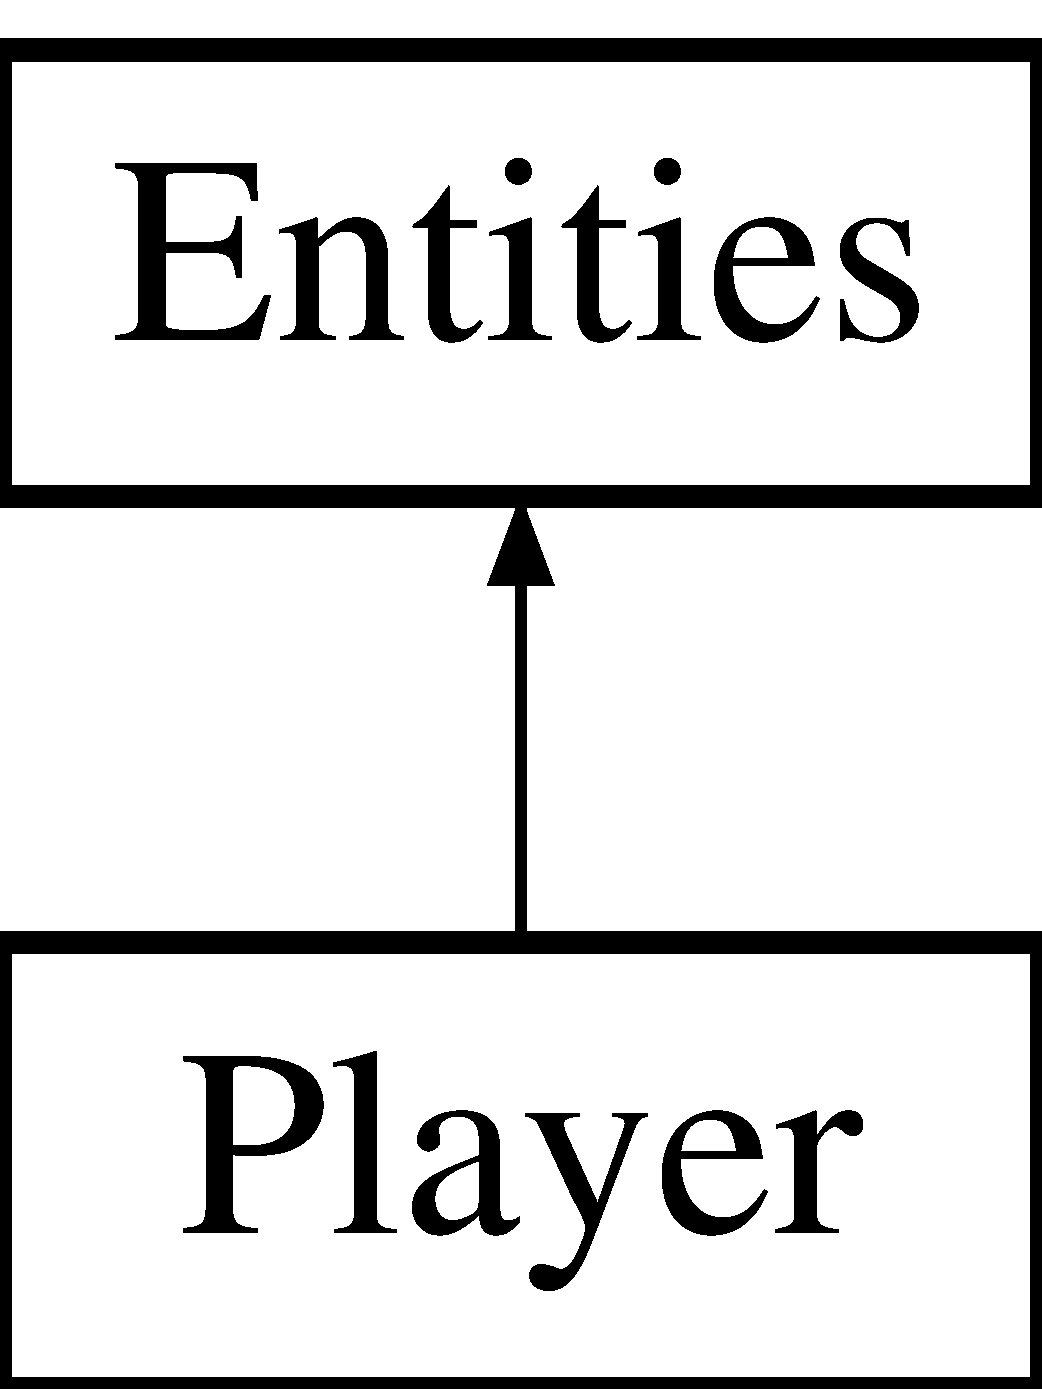
\includegraphics[height=2.000000cm]{classPlayer}
\end{center}
\end{figure}
\subsection*{Public Member Functions}
\begin{DoxyCompactItemize}
\item 
\hyperlink{classPlayer_affe0cc3cb714f6deb4e62f0c0d3f1fd8}{Player} ()
\item 
\hyperlink{classPlayer_a590f9fa9624d8734027fa2b290fa909e}{Player} (sf\-::\-Vector2f pos)
\item 
\hyperlink{classPlayer_ad2d6910c46e7fdf375870da47ae3db5f}{Player} (float px, float py)
\item 
\hyperlink{classPlayer_a749d2c00e1fe0f5c2746f7505a58c062}{$\sim$\-Player} ()
\item 
void \hyperlink{classPlayer_a01c63b9632f8a4f679f2e4cd704f14b9}{set\-Jump\-Time} (float time)
\item 
float \hyperlink{classPlayer_a9165dbc42a8d434d4eb0c64251305855}{get\-Jump\-Time} () const 
\item 
void \hyperlink{classPlayer_aa04cc1ac4ae2b43bfb841929e3d59315}{set\-Jump\-Height} (int height)
\item 
int \hyperlink{classPlayer_a41384c619c72d9cfd1ad6a354e917f8e}{get\-Jump\-Height} () const 
\item 
void \hyperlink{classPlayer_af7dc81f2576b432bc20e4040bb111422}{move} (sf\-::\-Vector2f movement)
\end{DoxyCompactItemize}


\subsection{Constructor \& Destructor Documentation}
\hypertarget{classPlayer_affe0cc3cb714f6deb4e62f0c0d3f1fd8}{\index{Player@{Player}!Player@{Player}}
\index{Player@{Player}!Player@{Player}}
\subsubsection[{Player}]{\setlength{\rightskip}{0pt plus 5cm}Player\-::\-Player (
\begin{DoxyParamCaption}
{}
\end{DoxyParamCaption}
)}}\label{classPlayer_affe0cc3cb714f6deb4e62f0c0d3f1fd8}
\hypertarget{classPlayer_a590f9fa9624d8734027fa2b290fa909e}{\index{Player@{Player}!Player@{Player}}
\index{Player@{Player}!Player@{Player}}
\subsubsection[{Player}]{\setlength{\rightskip}{0pt plus 5cm}Player\-::\-Player (
\begin{DoxyParamCaption}
\item[{sf\-::\-Vector2f}]{pos}
\end{DoxyParamCaption}
)}}\label{classPlayer_a590f9fa9624d8734027fa2b290fa909e}
\hypertarget{classPlayer_ad2d6910c46e7fdf375870da47ae3db5f}{\index{Player@{Player}!Player@{Player}}
\index{Player@{Player}!Player@{Player}}
\subsubsection[{Player}]{\setlength{\rightskip}{0pt plus 5cm}Player\-::\-Player (
\begin{DoxyParamCaption}
\item[{float}]{px, }
\item[{float}]{py}
\end{DoxyParamCaption}
)}}\label{classPlayer_ad2d6910c46e7fdf375870da47ae3db5f}
\hypertarget{classPlayer_a749d2c00e1fe0f5c2746f7505a58c062}{\index{Player@{Player}!$\sim$\-Player@{$\sim$\-Player}}
\index{$\sim$\-Player@{$\sim$\-Player}!Player@{Player}}
\subsubsection[{$\sim$\-Player}]{\setlength{\rightskip}{0pt plus 5cm}Player\-::$\sim$\-Player (
\begin{DoxyParamCaption}
{}
\end{DoxyParamCaption}
)}}\label{classPlayer_a749d2c00e1fe0f5c2746f7505a58c062}


\subsection{Member Function Documentation}
\hypertarget{classPlayer_a41384c619c72d9cfd1ad6a354e917f8e}{\index{Player@{Player}!get\-Jump\-Height@{get\-Jump\-Height}}
\index{get\-Jump\-Height@{get\-Jump\-Height}!Player@{Player}}
\subsubsection[{get\-Jump\-Height}]{\setlength{\rightskip}{0pt plus 5cm}int Player\-::get\-Jump\-Height (
\begin{DoxyParamCaption}
{}
\end{DoxyParamCaption}
) const}}\label{classPlayer_a41384c619c72d9cfd1ad6a354e917f8e}
\hypertarget{classPlayer_a9165dbc42a8d434d4eb0c64251305855}{\index{Player@{Player}!get\-Jump\-Time@{get\-Jump\-Time}}
\index{get\-Jump\-Time@{get\-Jump\-Time}!Player@{Player}}
\subsubsection[{get\-Jump\-Time}]{\setlength{\rightskip}{0pt plus 5cm}float Player\-::get\-Jump\-Time (
\begin{DoxyParamCaption}
{}
\end{DoxyParamCaption}
) const}}\label{classPlayer_a9165dbc42a8d434d4eb0c64251305855}
\hypertarget{classPlayer_af7dc81f2576b432bc20e4040bb111422}{\index{Player@{Player}!move@{move}}
\index{move@{move}!Player@{Player}}
\subsubsection[{move}]{\setlength{\rightskip}{0pt plus 5cm}void Player\-::move (
\begin{DoxyParamCaption}
\item[{sf\-::\-Vector2f}]{movement}
\end{DoxyParamCaption}
)\hspace{0.3cm}{\ttfamily [virtual]}}}\label{classPlayer_af7dc81f2576b432bc20e4040bb111422}


Reimplemented from \hyperlink{classEntities_a83e21f073e6792a036b9bd9388b0a083}{Entities}.

\hypertarget{classPlayer_aa04cc1ac4ae2b43bfb841929e3d59315}{\index{Player@{Player}!set\-Jump\-Height@{set\-Jump\-Height}}
\index{set\-Jump\-Height@{set\-Jump\-Height}!Player@{Player}}
\subsubsection[{set\-Jump\-Height}]{\setlength{\rightskip}{0pt plus 5cm}void Player\-::set\-Jump\-Height (
\begin{DoxyParamCaption}
\item[{int}]{height}
\end{DoxyParamCaption}
)}}\label{classPlayer_aa04cc1ac4ae2b43bfb841929e3d59315}
\hypertarget{classPlayer_a01c63b9632f8a4f679f2e4cd704f14b9}{\index{Player@{Player}!set\-Jump\-Time@{set\-Jump\-Time}}
\index{set\-Jump\-Time@{set\-Jump\-Time}!Player@{Player}}
\subsubsection[{set\-Jump\-Time}]{\setlength{\rightskip}{0pt plus 5cm}void Player\-::set\-Jump\-Time (
\begin{DoxyParamCaption}
\item[{float}]{time}
\end{DoxyParamCaption}
)}}\label{classPlayer_a01c63b9632f8a4f679f2e4cd704f14b9}


The documentation for this class was generated from the following files\-:\begin{DoxyCompactItemize}
\item 
\hyperlink{entities_8hpp}{entities.\-hpp}\item 
\hyperlink{entities_8cpp}{entities.\-cpp}\end{DoxyCompactItemize}

\chapter{File Documentation}
\hypertarget{entities_8cpp}{\section{entities.\-cpp File Reference}
\label{entities_8cpp}\index{entities.\-cpp@{entities.\-cpp}}
}
{\ttfamily \#include \char`\"{}entities.\-h\char`\"{}}\\*

\hypertarget{entities_8h}{\section{entities.\-h File Reference}
\label{entities_8h}\index{entities.\-h@{entities.\-h}}
}
{\ttfamily \#include $<$S\-F\-M\-L/\-System.\-hpp$>$}\\*
{\ttfamily \#include $<$S\-F\-M\-L/\-Graphics.\-hpp$>$}\\*
\subsection*{Classes}
\begin{DoxyCompactItemize}
\item 
class \hyperlink{classEntities}{Entities}
\begin{DoxyCompactList}\small\item\em The entities class. \end{DoxyCompactList}\item 
class \hyperlink{classPlayer}{Player}
\end{DoxyCompactItemize}

\hypertarget{game_8cpp}{\section{game.\-cpp File Reference}
\label{game_8cpp}\index{game.\-cpp@{game.\-cpp}}
}
{\ttfamily \#include $<$iostream$>$}\\*
{\ttfamily \#include \char`\"{}game.\-hpp\char`\"{}}\\*

\hypertarget{game_8h}{\section{game.\-h File Reference}
\label{game_8h}\index{game.\-h@{game.\-h}}
}
{\ttfamily \#include $<$S\-F\-M\-L/\-System.\-hpp$>$}\\*
{\ttfamily \#include $<$S\-F\-M\-L/\-Window.\-hpp$>$}\\*
{\ttfamily \#include $<$S\-F\-M\-L/\-Graphics.\-hpp$>$}\\*
{\ttfamily \#include \char`\"{}entities.\-h\char`\"{}}\\*
\subsection*{Classes}
\begin{DoxyCompactItemize}
\item 
class \hyperlink{classGame}{Game}
\end{DoxyCompactItemize}

\hypertarget{linefinder_8cpp}{\section{linefinder.\-cpp File Reference}
\label{linefinder_8cpp}\index{linefinder.\-cpp@{linefinder.\-cpp}}
}
{\ttfamily \#include \char`\"{}linefinder.\-hpp\char`\"{}}\\*
{\ttfamily \#include $<$utility$>$}\\*
{\ttfamily \#include $<$opencv2/core/core.\-hpp$>$}\\*
{\ttfamily \#include $<$opencv2/highgui/highgui.\-hpp$>$}\\*
{\ttfamily \#include $<$opencv2/imgproc/imgproc.\-hpp$>$}\\*
{\ttfamily \#include $<$opencv2/imgproc.\-hpp$>$}\\*
{\ttfamily \#include $<$play.\-hpp$>$}\\*

\hypertarget{linefinder_8hpp}{\section{linefinder.\-hpp File Reference}
\label{linefinder_8hpp}\index{linefinder.\-hpp@{linefinder.\-hpp}}
}
{\ttfamily \#include $<$opencv2/opencv.\-hpp$>$}\\*
{\ttfamily \#include $<$fstream$>$}\\*
{\ttfamily \#include $<$vector$>$}\\*
\subsection*{Classes}
\begin{DoxyCompactItemize}
\item 
class \hyperlink{classLineFinder}{Line\-Finder}
\end{DoxyCompactItemize}

\hypertarget{main_8cpp}{\section{main.\-cpp File Reference}
\label{main_8cpp}\index{main.\-cpp@{main.\-cpp}}
}
{\ttfamily \#include $<$iostream$>$}\\*
{\ttfamily \#include $<$string$>$}\\*
{\ttfamily \#include $<$fstream$>$}\\*
{\ttfamily \#include $<$opencv2/opencv.\-hpp$>$}\\*
{\ttfamily \#include $<$opencv2/highgui/highgui.\-hpp$>$}\\*
{\ttfamily \#include $<$opencv2/core/core.\-hpp$>$}\\*
{\ttfamily \#include $<$Q\-Application$>$}\\*
{\ttfamily \#include \char`\"{}play.\-hpp\char`\"{}}\\*
{\ttfamily \#include \char`\"{}mainwindow.\-hpp\char`\"{}}\\*
\subsection*{Functions}
\begin{DoxyCompactItemize}
\item 
int \hyperlink{main_8cpp_a0ddf1224851353fc92bfbff6f499fa97}{main} (int argc, char $\ast$argv\mbox{[}$\,$\mbox{]})
\end{DoxyCompactItemize}


\subsection{Function Documentation}
\hypertarget{main_8cpp_a0ddf1224851353fc92bfbff6f499fa97}{\index{main.\-cpp@{main.\-cpp}!main@{main}}
\index{main@{main}!main.cpp@{main.\-cpp}}
\subsubsection[{main}]{\setlength{\rightskip}{0pt plus 5cm}int main (
\begin{DoxyParamCaption}
\item[{int}]{argc, }
\item[{char $\ast$}]{argv\mbox{[}$\,$\mbox{]}}
\end{DoxyParamCaption}
)}}\label{main_8cpp_a0ddf1224851353fc92bfbff6f499fa97}

\hypertarget{play_8cpp}{\section{play.\-cpp File Reference}
\label{play_8cpp}\index{play.\-cpp@{play.\-cpp}}
}
{\ttfamily \#include \char`\"{}play.\-hpp\char`\"{}}\\*
{\ttfamily \#include $<$iostream$>$}\\*
{\ttfamily \#include $<$fstream$>$}\\*
{\ttfamily \#include $<$vector$>$}\\*
{\ttfamily \#include $<$string$>$}\\*

\hypertarget{play_8hpp}{\section{play.\-hpp File Reference}
\label{play_8hpp}\index{play.\-hpp@{play.\-hpp}}
}
{\ttfamily \#include $<$string$>$}\\*
{\ttfamily \#include $<$vector$>$}\\*
{\ttfamily \#include \char`\"{}linefinder.\-hpp\char`\"{}}\\*
{\ttfamily \#include \char`\"{}game.\-hpp\char`\"{}}\\*
\subsection*{Classes}
\begin{DoxyCompactItemize}
\item 
class \hyperlink{classPlay}{Play}
\begin{DoxyCompactList}\small\item\em The \hyperlink{classPlay}{Play} class. \end{DoxyCompactList}\end{DoxyCompactItemize}

\hypertarget{README_8md}{\section{R\-E\-A\-D\-M\-E.\-md File Reference}
\label{README_8md}\index{R\-E\-A\-D\-M\-E.\-md@{R\-E\-A\-D\-M\-E.\-md}}
}

\addcontentsline{toc}{part}{Index}
\printindex
\end{document}
